\chapter{Radonová problematika}\label{navesti:radon}
Radon je bezbarvý, nereaktivní plyn, je bez chuti a zápachu \cite{wiki_radon}. Vzniká přeměnou z radia. Nejvýznamnějším radionuklidem je \ce{^{222}Rn} z uranové řady vznikající z \ce{^{226}Ra} s poločasem přeměny 3,82 dne. Mluví-li se o radonu jako radionuklidu, pak je míněn právě \ce{^{222}Rn}. V této práci dále uvažujeme pouze tento radionuklid. Radon způsobuje přibližně 50~\% celkového ozáření obyvatelstva~\cite{SURO}.

V tab.~\ref{tab:radon_dcery} jsou uvedeny krátkodobé dceřinné produkty radonu s jejich poločasy přeměny a způsobem přeměny. Pomocí nich se radon může měřit a právě ony mají hlavní podíl na ozařování obyvatelstva.
\begin{table}[H]
    \centering
    \caption{Krátkodobé dceřinné produkty radonu, jejich poločasy přeměny a způsob dominantní přeměny~\cite{SURO}.}
    \label{tab:radon_dcery}
    \begin{tabular}{lll}
        \toprule
        RN& $T_{1/2}$ &přeměna\\
        \midrule
        \ce{^{218}Po}& \SI{3.05}{min} & $\alpha$\\
        \ce{^{214}Pb}& \SI{26.8}{min} & $\beta$\\
        \ce{^{214}Bi}& \SI{19.7}{min} & $\beta$\\
        \ce{^{214}Po}& \SI{164}{\mu s} & $\alpha$\\
        \bottomrule
    \end{tabular}
\end{table}

Radon vzniká v geologickém podloží, ze kterého se dostává do obytných budov. Pokud se v budovách dostatečně nevětrá, nebo pokud je přísun radonu z podloží do budovy neobvykle vysoký, pak může OAR (objemová aktivita radonu, nazývaná též koncentrace radonu vyjádřená v \si{Bq/m^3}) uvnitř budovy dosahovat velikých hodnot, což může z dlouhodobého hlediska ohrožovat zdraví obyvatel. Pro rozhodnutí, co je a není příliš vysoká hodnota OAR, vyhláška o radiační ochraně~\cite{vyhlaska} stanovuje referenční hodnotu \SI{300}{Bq/m^3}. Při jejím překročení by měl vlastník budovy v rámci optimalizace radiační ochrany přikročit k úpravě užívání budovy (více větrat) nebo k provedení ozdravných opatření (odčerpávání radonu z půdního vzduchu). Informace o působení radonu na lidské zdraví lze dohledat např. na stránkách Státního ústavu radiační ochrany, v. v. i. (SÚRO),~\cite{SURO}.

Z předchozího textu plyne, že je potřeba koncentraci radonu v budovách dostatečně přesně měřit. Detektory radonu rozdělujeme na integrální a kontinuální. Integrální poskytují jednu průměrnou hodnotu OAR za celou dobu měření, ale nepotřebují napájení. Naopak kontinuální detektory měří průběh OAR v čase a potřebují napájení. 

Mezi nejvíce používané integrální detektory radonu pro měření v budovách se řadí stopové detektory a elektretové ionizační komory. Stopové detektory se užívají pro dlouhodobější měření (zpravidla roční), elektretové se využívají při kratších měření (týdenní, dvoutýdenní). V rámci této práce jsem ani s jedním z těchto typů detektorů nepracoval, a proto o nich zde neuvádím podrobnější informace (ty lze opět dohledat v \cite{SURO}). V kapitole~\ref{navesti:rovnovaznaMereni} jsem však využíval OAR naměřené elektretovými detektory.

V případě kontinuálních detektorů se používá termín kontinuální monitory radonu, protože tak nedochází ke zmatení názvosloví. Kontinuální monitory radonu se totiž dělí nejenom podle typu použitého detektoru (polovodičový, ionizační komora), ale i podle nasávání vzduchu, způsobu vyhodnocování naměřených dat, atd. V následujícím odstavci jsou uvedeny parametry dvou kontinuálních monitorů, které jsem při měření používal.

V odstavci~\ref{navesti:radon_zdroje} jsou uvedené základní informace o průtočném radonovém zdroji, který jsem používal při měřeních.

\section{Použité kontinuální monitory radonu}
\subsection{TERA sondy}
Jedná se o monitory s polovodičovým detektorem. Nasávání vzduchu je prováděno difúzně. Mají dva režimy měření:
\begin{labeling}{RaA+RaC}
    \item[RaA] rychlejší, ale méně přesný způsob. OAR se počítá pouze z naměřených impulzů od alfa částic vznikajících při přeměně příslušející \ce{^{218}Po}.
    \item[RaA+RaC] pomalejší, ale přesnější způsob. OAR se počítá z impulzů od alfa částic vznikajících při přeměnách \ce{^{218}Po} i \ce{^{214}Po}.
\end{labeling}

Sondy neustále měří a zpracovávají výsledky v čtyř minutových intervalech, z kterých každou hodinu počítají koncentraci radonu (pomocí klouzavého průměru). Tyto hodinové hodnoty lze po skončení měření vyčíst. Některé verze sond mají displej, na němž je vidět tato hodinová hodnota (aktuální v daném čase) a také dlouhodobá koncentrace radonu (24 hodinový klouzavý průměr). \cite{tera}

Parametry uváděné výrobcem tohoto kontinuálního monitoru radonu jsou v tab.~\ref{tab:radon_tera}, v obr.~\ref{fig:radon_tera} je TERA sonda zobrazena. Tyto monitory byly využity jako primární měřidlo OAR při mých měřeních. Při všech měřeních byl používán režim RaA+RaC.

O TERA sondách je z praxe známo, že jsou značně nepřesné a OAR naměřené několika sondami se mohou lišit až třeba o 40~\%. Proto bylo potřeba před samotným měřeními udělat se sondami srovnávací měření s nějakým osvědčeným monitorem radonu, např. AlphaGuardem~\cite{alphaguard}, aby se mohly zavádějící hodnoty OAR opravit. Toto srovnávací měření je rozebráno v podkapitolce~\ref{navesti:dynMer_TERA}.

\subsubsection{Určení nejistot naměřených OAR}
Jak již bylo řečeno, TERA sondy zapisují průměrnou hodnotu OAR každou hodinu. Spolu s OAR jsou zapisovány i naměřené počty impulzů v jednotlivých diskriminačních oknech, která mají TERA sondy nastaveny pro rozlišení impulzů: do druhého diskriminačního okna spadají impulzy od \ce{^{218}Po} (\SI{6}{MeV}), do třetího od \ce{^{214}Po} (\SI{7.69}{MeV}), do prvního a čtvrtého impulzy od ostatních energií, jenž nás nezajímají. Díky tomu je možné vypočítat nejistotu naměřeného počtu impulzů náležejících \ce{^{218}Po} a \ce{^{214}Po}. Označme tento počet impulzů jako $n$. Počet zaznamenaných impulsů se řídí Poissonovým rozdělením, a proto pro směrodatnou odchylku $n$ máme:
\begin{equation}
    \sigma_n=\sqrt{n}\,.
    \label{eq:radon_n_odchylka}
\end{equation}
Dle tab.~\ref{tab:radon_tera} je průměrná citlivost měření \SI{0.25}{(imp/hod)/(Bq/m^3)}, ale při zkoušení vypočítání citlivosti z naměřených dat (jako podíl $n$ a OAR) mi pro každou zaznamenanou hodnotu vycházela citlivost jinak. To znamená, že kalibrace sond je nějaká funkce OAR. Proto je přesnější vypočítat si citlivost pro každou hodnotu z naměřených dat místo používání tabelované hodnoty.

Při určování nejistoty OAR vycházíme ze znalosti $n$ pro danou OAR:
\begin{align}
    \sigma_{OAR}&=\frac{\sigma_n}{c}=\frac{\sqrt{n}\cdot OAR}{n}=\frac{OAR}{\sqrt{n}}\,,
    \label{eq:radon_OAR_odchylka}
\end{align}
kde $c$ je označení citlivosti.

Pro úplnost zde ještě uvadíme definici citlivosti $c$:
\begin{equation}
    n=c\cdot OAR
    \label{eq:radon_citlivost}
\end{equation}

\subsection{CANARY měřáky}
Také se jedná o monitory s polovodičovým detektorem zapisující hodnotu OAR každou druhou hodinu. Tato hodnota je průměrem ze dvou hodin měření, přičemž čas zápisu do paměti monitoru je uprostřed tohoto měření. Využívají taktéž pasivního difúzní nasávání vzduchu. Jsou to kompaktní malá zařízení k rychlému určení OAR v zkoumaném objektu. 

Parametry uváděné výrobcem jsou v tab.~\ref{tab:radon_canary}. V obr.~\ref{fig:radon_canary} je CANARY měřák k nahlédnutí. CANARY měřáky byly použity jako záložní měřidlo OAR.
\begin{figure}[H]
    \centering
    \begin{subfigure}[b]{0.35\textwidth}
        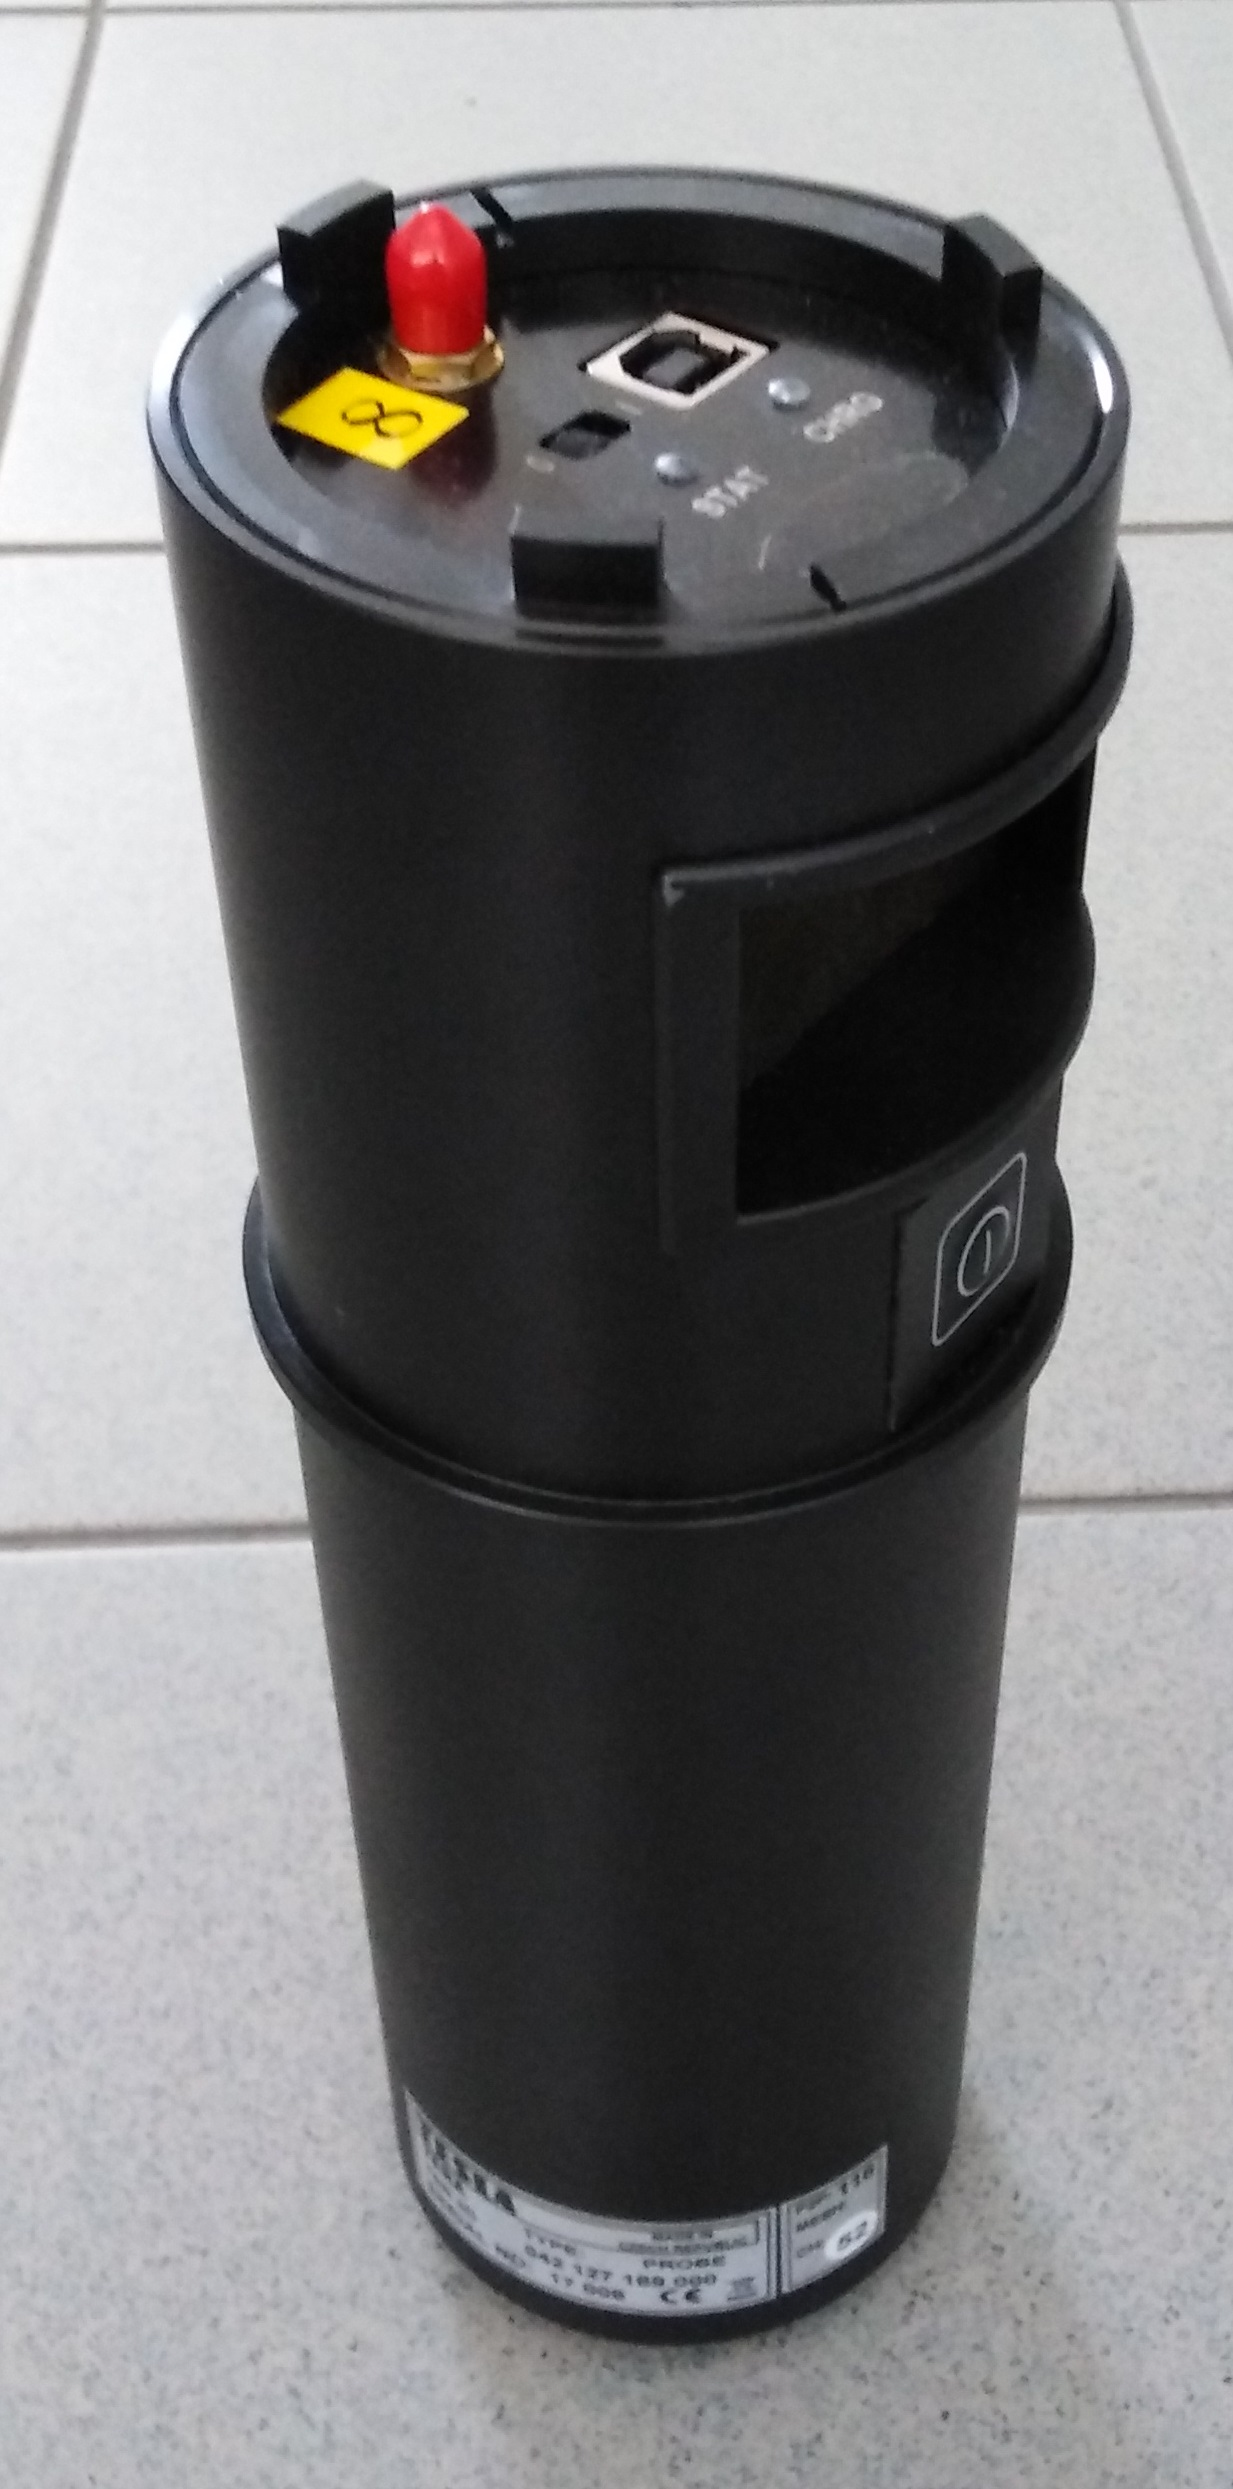
\includegraphics[width=.9\textwidth]{tera.jpg}
        \caption{}
        \label{fig:radon_tera}
    \end{subfigure}
    \begin{subfigure}[b]{0.3\textwidth}
        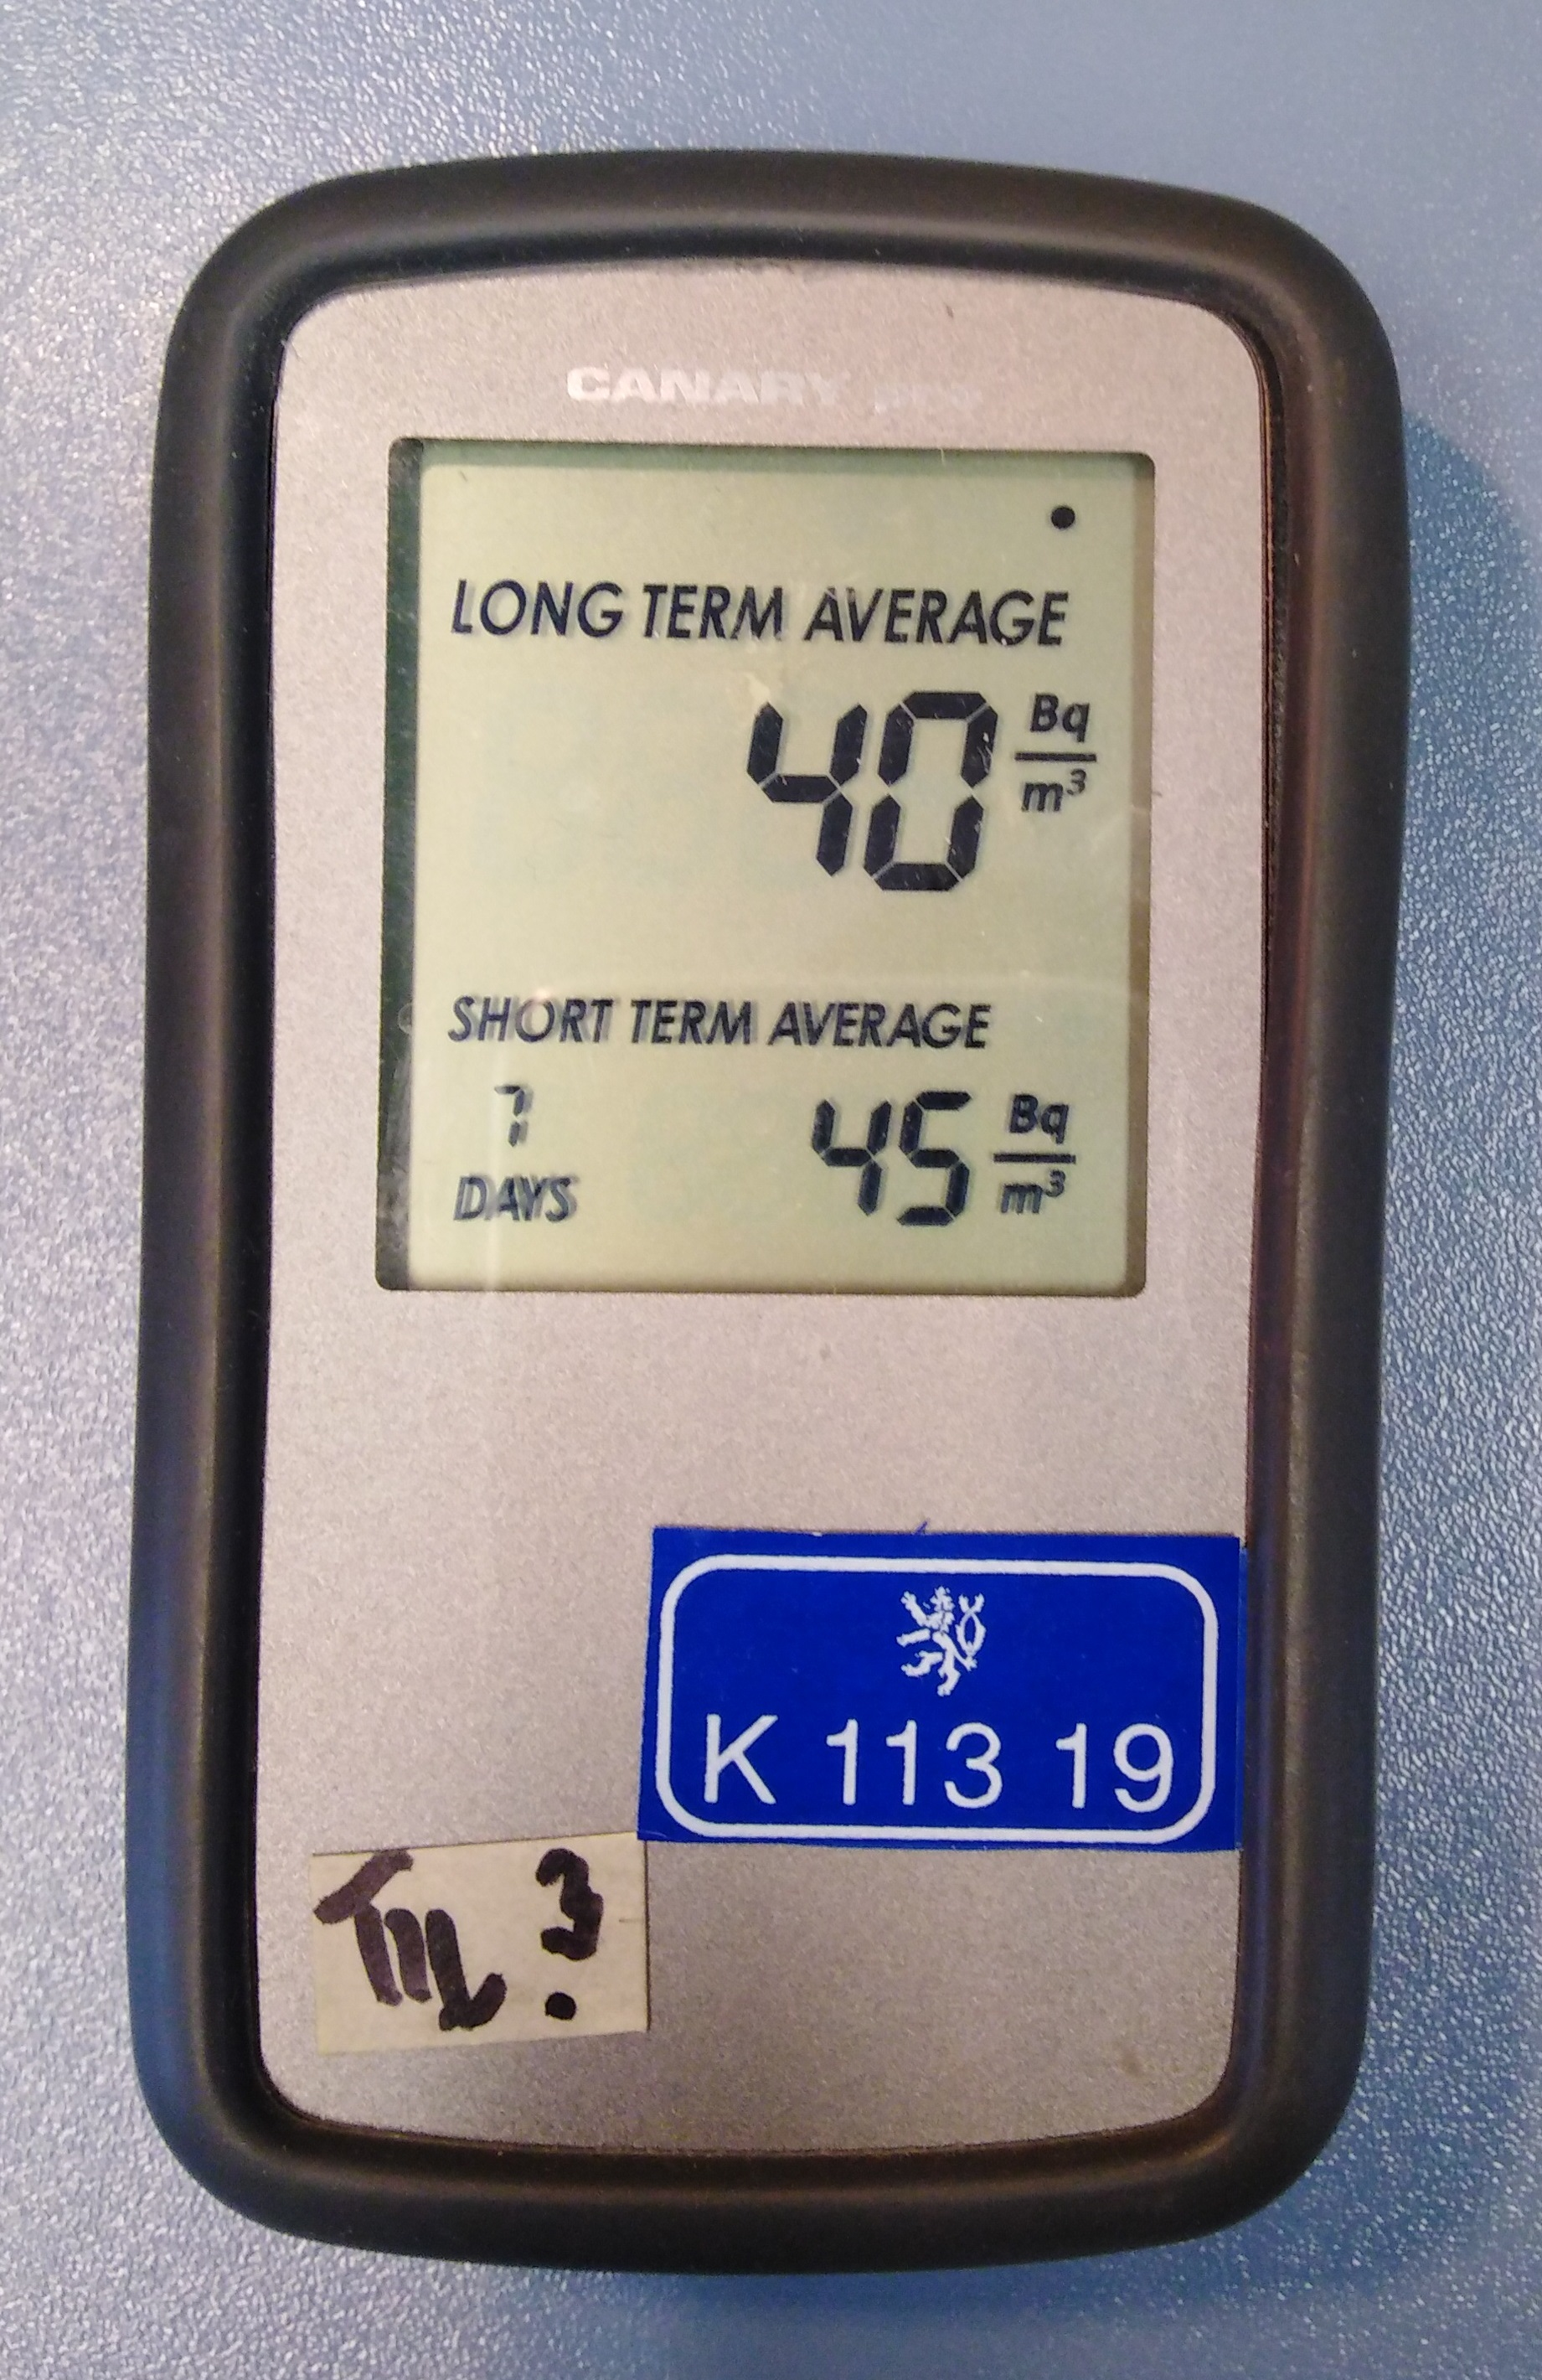
\includegraphics[width=.9\textwidth]{canary.jpg}
        \caption{}
        \label{fig:radon_canary}
    \end{subfigure}
    \caption{V (a) je TERA sonda (verze s displejem), v (b) CANARY měřák.}
\end{figure}

\begin{table}[H]
    \centering
    \caption{Technické parametry CANARY měřáků, novým názvem Corentium Home Airthings~\cite{canary}.}
    \label{tab:radon_canary}
\begin{tabular}{ll}
    \toprule
Baterka                   & 3 AAA alkalinové baterie (LR03)        \\
                              & dvouroční životnost baterie                   \\
Rozměry                    & 120 $\times$ 69 $\times$ 25,5 \si{mm^3}                     \\
Hmotnost                        & 130 g                                  \\
Měří při          & teplota: +4\degree C to +40\degree C            \\
                              & relativní vlhkost: $<$ 85 \%           \\
Měřící rozsah             & nejnižší detekční limit: \SI{0}{Bq/m^3}        \\
                              & horní limit displeje: \SI{9999}{Bq/m^3}        \\
\midrule
\multicolumn{2}{l}{\textbf{Přesnost při \SI{200}{Bq/m^3}:}} \\
\midrule
7 dní                        & 10 \%                                  \\
2 měsíce                      & 5 \%                  \\                
\bottomrule
\end{tabular}
\end{table}

\begin{table}[H]
    \centering
    \caption{Technické parametry TSR3D a TSR3 sond (neboli TERA sond)~\cite{tera}.}
    \label{tab:radon_tera}
    \begin{tabular}{p{.55\textwidth}p{.45\textwidth}}
    \toprule
    Průměrná citlivost měření                                & \SI{0,25}{(imp/hod)/(Bq/m^3)}                                                       \\
                                                         & (metoda RaA+RaC; 15\degree C -- 30\degree C; rel. vlh. 20 \% -- 40 \%)               \\
Rozsah měření                                            & MDA až \SI{1e6}{Bq/m^3};                                                         \\
                                                         & MDA = \SI{100}{Bq/m^3} při 1 hodině měření nebo \SI{20}{Bq/m^3} při 24 hodinovém měření \\
Nejistota měření                                         & $<$ 13\% při \SI{300}{Bq/m^3} a 1 hodině měření;                           \\
                                                         & $<$ 3\% při \SI{300}{Bq/m^3} a 24 hodinovém měření                         \\
Objem měřící komory                                      & 0,176 \si{dm^3}                                                                 \\
Rychlost odezvy                                          & $<$ 30 minut (RaA); $<$ 3 hodiny (RaA + RaC)                  \\
Měřící algoritmus                                        & rychlý, měně přesný (počítáno z RaA)                                      \\
                                                         & pomalý, více přesný (počítáno z RaA+ RaC)                                 \\
Měření relativní vlhkosti                                & 10 – 90 \%                                                                \\
Měření teploty                                           & od -20\degree do +60\degree C                                              \\
%Radiové rozhraní                                         & 868 MHz                                                                    \\
%Max. počet prvků v měřící síti                           & 16                                                                        \\
Možnost použití opakovače pro zvětšení dosahu            & ano                                                                       \\
Interval čtení výsledků měření ze sondy                  & 240 – 65535 s (4 min – 18,2 hod)                                          \\
Interval uložení výsledků v sondě                        & 1 – 255 min, defaultně každou 1 hodinu                                    \\
Kapacita paměti výsledků v sondě (při autonomním měření) & 150 dní                                                                   \\
Napájení sondy                                           & Vnitřní nabíjecí akumulátor; nabíjení přes USB                            \\
Předpokládaná doba provozu po nabití                     & $>$ 1 rok                                                        \\
Indikace aktuální koncentrace radonu                     & krátkodobá (klouzavý průměr za 1 hodinu);                                  \\
                                                         & dlouhodobá (klouzavý průměr za 24 hodin)                                  \\
Rozměry                                                  & $\diameter$ 80 $\times$ 175 mm                                                   \\
%Vestavěný displej                                        & grafický, 128 $\times$ 64 bodů, jantarové podsvícení      \\      
\bottomrule
\end{tabular}
\end{table}

\section{Průtočné radonové zdroje typu RF 2000}\label{navesti:radon_zdroje}

Jedná se o kalibrované zdroje s deklarovanou aktivitou \ce{^{226}Ra} a radonovou výdejností. Radonová výdejnost je množství radonu, které se ze zdroje za pomoci čerpadla dostane ven za jednotku času, a udává se v jednotkách v \si{Bq/s}. Vzhled zdroje je k nahlédnutí v obr.~\ref{fig:radon_zdroj}.

Při měřeních jsem využíval dva zdroje tohoto typu, viz kapitola~\ref{navesti:dynamickaMereni}.
\begin{figure}[ht]
    \centering
    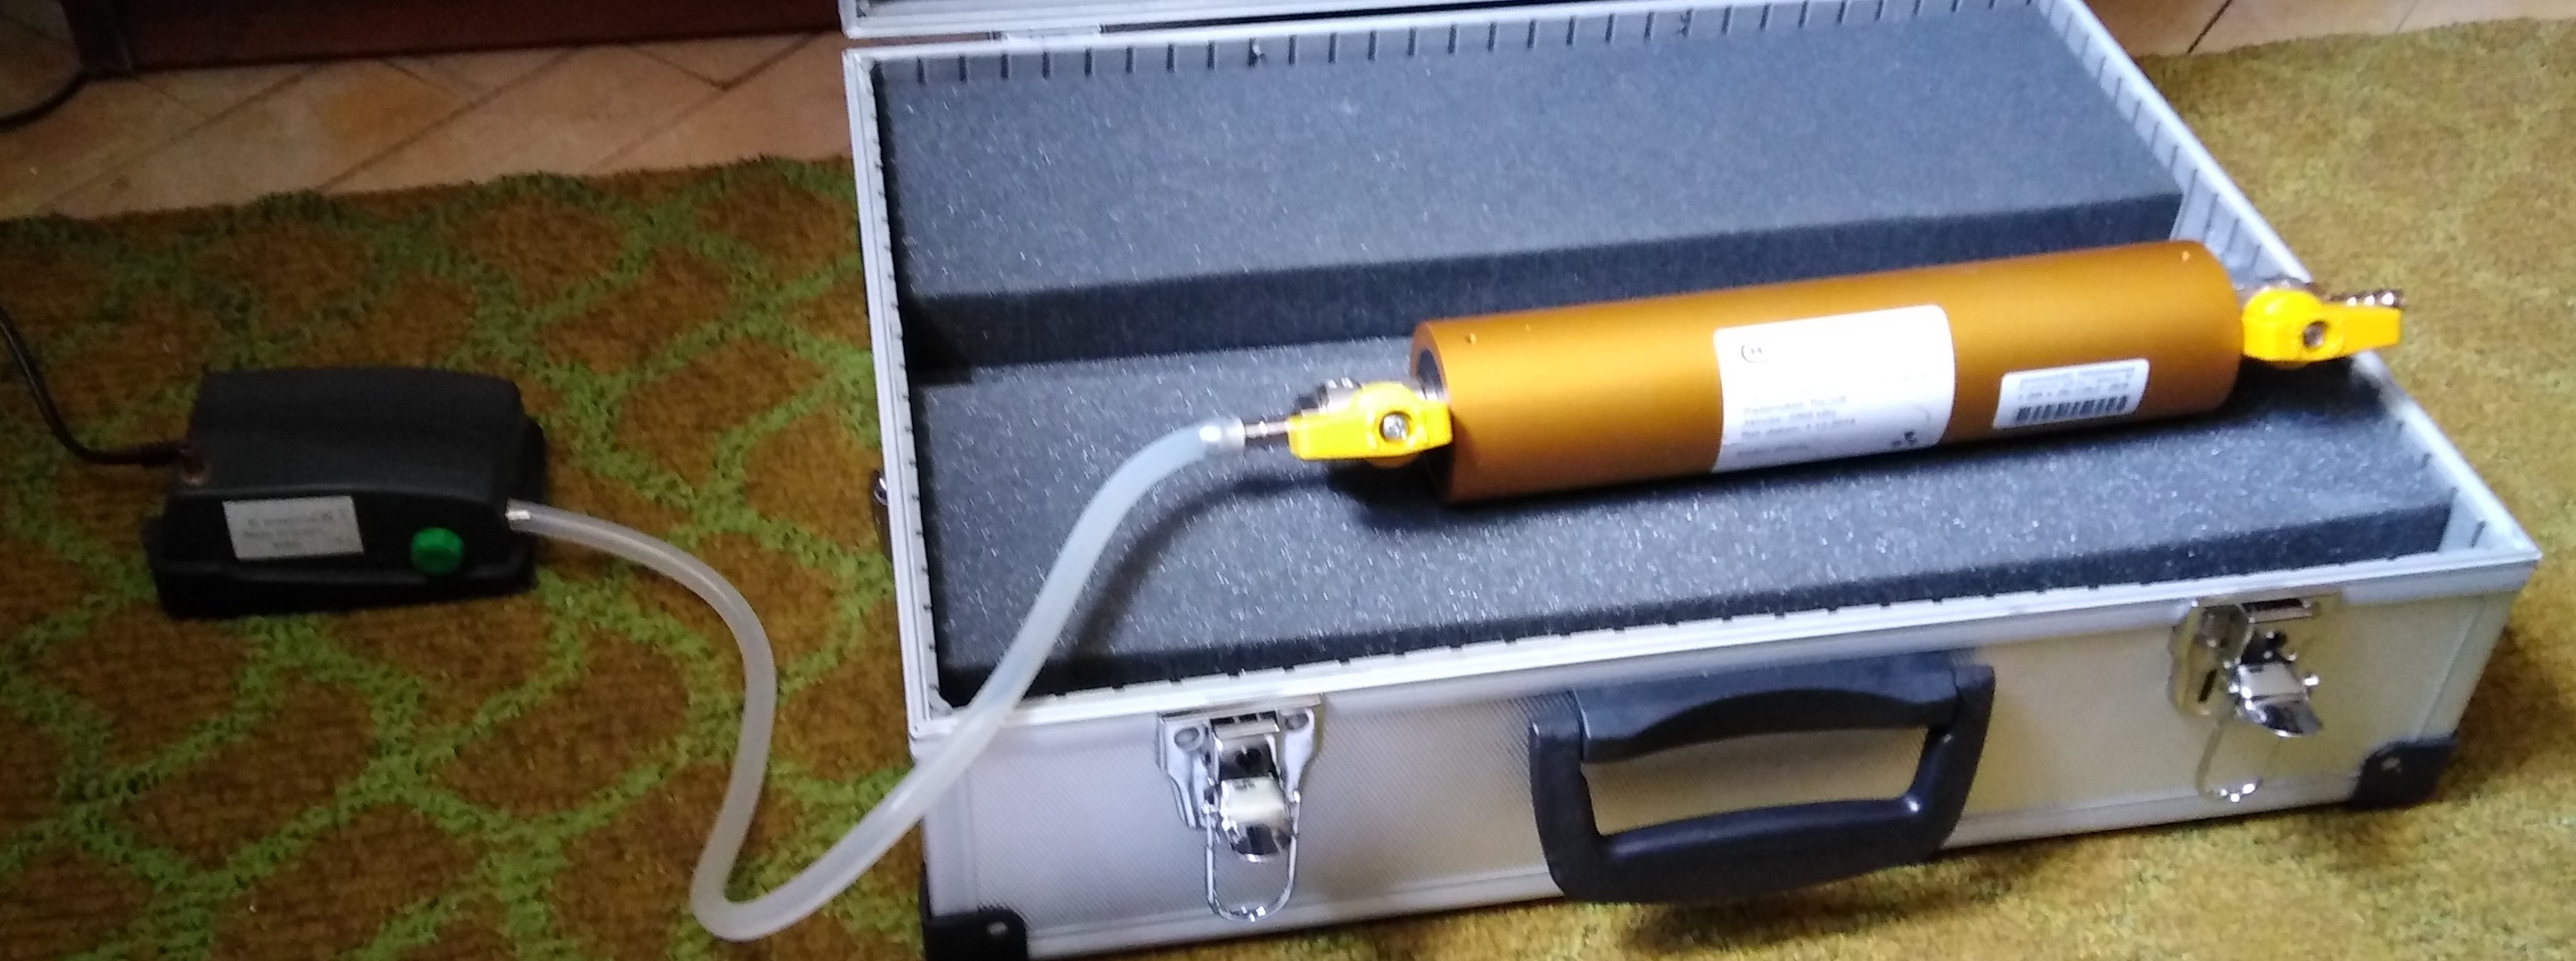
\includegraphics[width=0.85\textwidth]{zdroj.jpg}
    \caption{Průtočný zdroj typu RF 2000 s připojeným čerpadlem.}
    \label{fig:radon_zdroj}
\end{figure}
